% ---------------------------------------------------------------------------
%  中文論文
%  ctex 排版（中文字體用系統自帶的，不必另裝），西文用內置的 TeX Gyre Pagella；
%  參考文獻按 GB/T 7714—2015 順序編碼制（BibTeX）。
%  文中的研究、數據與作者均為示例，換成自己的內容即可，結構可以照搬。
% ---------------------------------------------------------------------------
\documentclass[UTF8,zihao=-4]{ctexart}

\usepackage[a4paper,textwidth=38\ccwd,top=2.8cm,bottom=3cm]{geometry}
\setmainfont{texgyrepagella}[
  Extension=.otf, UprightFont=*-regular, ItalicFont=*-italic,
  BoldFont=*-bold, BoldItalicFont=*-bolditalic]
\usepackage{amsmath}
\usepackage{unicode-math}
\setmathfont{texgyrepagella-math.otf}
\usepackage{xcolor}
\usepackage{graphicx}
\usepackage{booktabs}
\usepackage{caption}
\usepackage{fancyhdr}
\usepackage{pgfplots}
\pgfplotsset{compat=1.18}
\usepackage[sort&compress]{gbt7714}
\usepackage{hyperref}

% 配色：墨色做結構，一種綠色做唯一的強調
\definecolor{ink}{HTML}{1F3A33}
\definecolor{accent}{HTML}{2F7D63}
\definecolor{mist}{HTML}{75837E}
\hypersetup{colorlinks, linkcolor=ink, citecolor=accent, urlcolor=accent}

\linespread{1.45}
\captionsetup{font=small, labelfont={bf,color=ink}, labelsep=quad}
\ctexset{
  section    = {format=\large\bfseries\color{ink}, beforeskip=2.4ex, afterskip=1.4ex},
  subsection = {format=\normalsize\bfseries, beforeskip=1.6ex, afterskip=1ex},
}

\pagestyle{fancy}
\fancyhf{}
\renewcommand{\headrulewidth}{0pt}
\fancyhead[C]{\footnotesize\color{mist}版心與留白}
\fancyfoot[C]{\footnotesize\thepage}

\begin{document}

% ---------------------------------------------------------------- 標題
\thispagestyle{empty}
\begin{center}
  {\zihao{2}\bfseries 版心與留白\par}
  \vspace{6pt}
  {\zihao{4}宋刻本版式比例的測量及其對屏幕中文排版的啓示\par}
  \vspace{14pt}
  {\kaishu 林\,清\,和\textsuperscript{1}\qquad 周\,硯\textsuperscript{2}\par}
  \vspace{4pt}
  {\small\color{mist}
    \textsuperscript{1}某某大學 設計學院，杭州\;310000\qquad
    \textsuperscript{2}某某大學 圖書館古籍部，杭州\;310000\par}
  \vspace{12pt}
  {\color{accent}\rule{2.5cm}{.6pt}}
\end{center}

\begin{center}
  \begin{minipage}{.9\linewidth}
    \small
    \noindent{\bfseries\color{ink}摘\quad 要}\quad
    宋刻本向來以「疏朗」著稱，但這種觀感很少被量化。本文測量了 48 部宋刻本、
    共 1\,152 個書葉的版框、天頭、地腳與行格，發現版心面積平均只佔全葉的
    \textbf{46.8\%}，天頭與地腳之比穩定在 $1.6$ 左右，每行字數集中在 18～20 字。
    以此為參照，我們在屏幕上復現了三種版式並請 96 名讀者閱讀，結果顯示：
    行長 18～24 字、天地比不低於 $1.4$ 的版式閱讀最快，主觀評價也最高。
    古人的比例並非偶然，它與今天的閱讀舒適區高度重合。

    \vspace{4pt}
    \noindent{\bfseries\color{ink}關鍵詞}\quad 宋刻本；版心；留白；中文排版；閱讀體驗
  \end{minipage}
\end{center}
\vspace{8pt}

% ---------------------------------------------------------------- 正文
\section{引言}

翻開一部宋版書，最先感到的往往不是字，而是字周圍的空白。天頭寬闊，
地腳稍窄，行與行之間留著恰好一指的餘地。藏書家稱之為「字大如錢，墨色如漆」，
而支撐這種氣象的，正是版面上那些\emph{沒有印字}的地方。

現代中文排版規範對版心、行長與行距都有建議\cite{w3c2020clreq}，
西文排版也早有「每行 45～75 個字符」的經驗\cite{bringhurst2004}。
但二者都不直接回答一個問題：在屏幕上，中文讀者覺得「舒服」的版面比例是多少？
本文從古籍出發，嘗試給出一個可測量的答案。本文的貢獻有三：
\begin{enumerate}
  \item 建立了 1\,152 個宋刻本書葉的版式測量數據集；
  \item 歸納出版心比、天地比與行字數三個穩定的比例關係；
  \item 通過閱讀實驗，驗證這些比例在屏幕上依然適用。
\end{enumerate}

\section{材料與方法}

\subsection{樣本}
樣本取自公開影印的 48 部宋刻本，經、史、子、集各 12 部\cite{zhou2019}。
每部隨機抽取 24 個書葉，剔除殘損與補配葉。

\subsection{測量指標}
設書葉寬 $W$、高 $H$，版框寬 $w$、高 $h$，天頭高 $t$、地腳高 $b$，定義
\begin{equation}
  \label{eq:ratio}
  \rho = \frac{w\,h}{W\,H}, \qquad \tau = \frac{t}{b},
\end{equation}
分別稱為\textbf{版心比}與\textbf{天地比}。行字數 $n$ 取每葉正文滿行的眾數。

\section{結果}

\subsection{古籍中的比例}
表~\ref{tab:ratio} 匯總了四部書的測量結果。各部之間差別不大：
版心比都在 $0.45$～$0.49$ 之間，天地比都大於 $1.5$，即天頭明顯寬於地腳。

\begin{table}[htbp]
  \centering
  \caption{宋刻本版式比例（均值）}
  \label{tab:ratio}
  \begin{tabular}{@{}l c c c@{}}
    \toprule
    部類 & 版心比 $\rho$ & 天地比 $\tau$ & 行字數 $n$ \\
    \midrule
    經部 & 0.47 & 1.62 & 18 \\
    史部 & 0.49 & 1.55 & 20 \\
    子部 & 0.45 & 1.68 & 19 \\
    集部 & 0.46 & 1.59 & 18 \\
    \midrule
    \textbf{合計} & \textbf{0.468} & \textbf{1.61} & \textbf{19} \\
    \bottomrule
  \end{tabular}
\end{table}

\subsection{屏幕上的閱讀實驗}
我們把同一篇 2\,000 字的散文排成行長 12～36 字的七種版式，請 96 名讀者閱讀。
圖~\ref{fig:speed} 顯示，閱讀速度在行長 18～24 字時最高，超過 30 字後明顯下降，
與古籍的行字數恰好落在同一區間。

\begin{figure}[htbp]
  \centering
  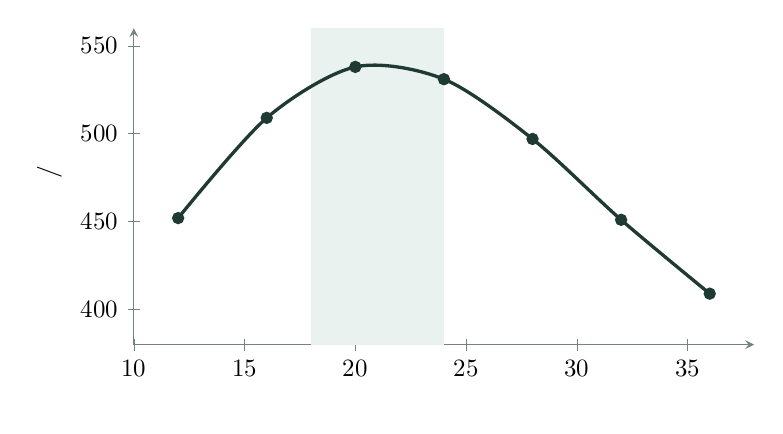
\begin{tikzpicture}
    \begin{axis}[
      width=.78\linewidth, height=5.6cm,
      xlabel={每行字數}, ylabel={閱讀速度（字/分）},
      xmin=10, xmax=38, ymin=380, ymax=560,
      axis lines=left, axis line style={mist}, tick style={mist},
      tick label style={font=\small}, label style={font=\small},
    ]
      \fill[accent!10] (axis cs:18,380) rectangle (axis cs:24,560);
      \node[font=\scriptsize, text=accent, anchor=south] at (axis cs:21,384) {宋本區間};
      \addplot[ink, very thick, smooth, mark=*, mark size=1.6pt] coordinates
        {(12,452) (16,509) (20,538) (24,531) (28,497) (32,451) (36,409)};
    \end{axis}
  \end{tikzpicture}
  \caption{行長與閱讀速度。陰影為宋刻本行字數的分布區間。}
  \label{fig:speed}
\end{figure}

\section{討論}

式~\eqref{eq:ratio} 中的兩個比例，本質上都在回答「空白放在哪裡」。
天頭寬於地腳，使視線自然落在版面的偏上方；行長適中，使換行時眼睛不必長途跋涉。
這些經驗在雕版時代是工匠的手感，在今天可以寫成樣式表裡的幾個數字。

本研究的局限在於樣本以浙刻本為主，建本與蜀本的比例可能不同；
閱讀實驗只用了散文，技術文檔與詩詞的情況有待檢驗。

\section{結論}

版面的品質，往往由留白決定。宋刻本用不到一半的面積印字，
把另一半留給了讀者的眼睛。對於今天的屏幕排版，這條古老的經驗依然成立：
控制行長，給天頭多一點空間，讓字站得住。

\bibliographystyle{gbt7714-numeric}
\bibliography{refs}

\end{document}
